
%\subsubsection{ECal Trigger overview}


The proposed trigger system is nearly deadtimeless. 
 The trigger logic will search for a time coincidence between two clusters in opposite halves of ECal for ($e^+e^-$) trigger and two MIP signatures in opposite halves of ECal and at least in the first 2 layers of the muon hodoscopes for ($\mu^+\mu^-$) trigger. The coincidence time window is programmable with 4ns resolution. The maximum trigger decision time (latency) is currently set to 3 $\mu$s for Level 1. That value is defined by the SVT readout APV25 chip.

The Trigger Supervisor generates all necessary signals, and controls the entire DAQ system readout through the Trigger Interface units. The Trigger Interface (TI) units installed in every crate participate in the readout process. The trigger supervisor can apply deadtime if necessary, for example on a 'busy' or 'full' condition from front-end electronics. The system is free-running and driven by a 250MHz global clock. The maximum trigger accept rate is 50 KHz.

The first stage components of the trigger logic are incorporated into FPGAs of the Flash ADC board's, while the final decision is made in a Crate Trigger Processors (CTPs) and  Sub-System Processor (SSP) . As described above, 
FADC sends 13-bit pulse energy and time information to CTP. With available 3-bit time information, CTP can in principal look for coincidence between different channels in 4 ns time window. For the HPS L1 trigger formation, the time window for channel coincidence will be set to 8 ns.

\begin{figure}[t]
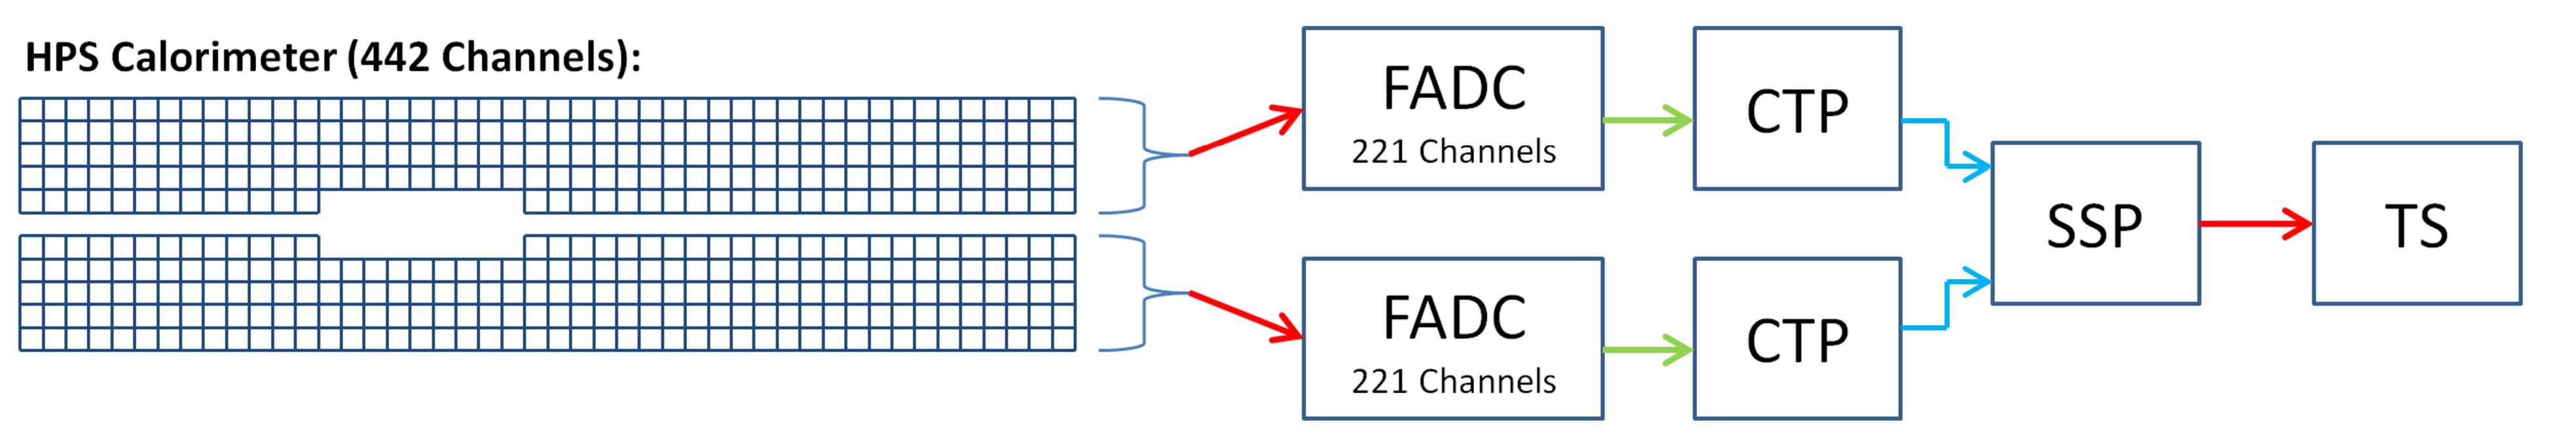
\includegraphics[scale=0.25]{daq_trigger/figures/hps_trigger_cal}
\caption{\small{ECAL trigger logic. FADC - Jlab Flash ADC, CTP - Crate Trigger Processor, SSP - Sub-System Processor, TS - Trigger Superviser.}}
\label{fig:hps_trigger_cal}
\end{figure}

{\bf ECal $e^+e^-$ Trigger} 

The trigger system for ECal can be broken down into the following 3 sections, see Figure \ref{fig:hps_trigger_cal}:
 \begin{itemize}
 \item FADC (pulse finding): Samples the detector channel to find pulses above the preset trigger threshold. Pulse energy and times are sent to CTP
 \item CTP (cluster finding): Searches FADC pulses (from half of calorimeter) to find clusters. Cluster energy, time, and hit pattern sent to SSP
 \item SSP (cluster pair finding): Searches CTP clusters (from top and bottom) to find cluster pairs and creates the trigger. Trigger cuts on pairs decide final trigger.
 \end{itemize}
 
The algorithm used for cluster finding makes use the parallel processing nature of FPGAs by simultaneously searching for 125 clusters up to 3x3 in size across the calorimeter crystal array (see Figure~\ref{fig:hps_trigger_3x3}).  
A Cluster Processor (CP) algorithm performs the following tasks:

\begin{itemize}
\item Adds energy from hits together for every 3x3 square of channels in ECal
\item Hits are added together if they occur (leading edge) within a programmable number of clock cycles of each other (4 ns steps)
\item If 3x3 energy sum $\ge$  the programmable cluster energy threshold, CTP reports cluster parameters (time, energy, position and 3x3 hit pattern) to the Sub-System processor. 
\end{itemize}

Every 4ns the CTP evaluates all hits in its half of the calorimeter. A programmable time window is used to allow hits that are out of time with each other be considered as part of a cluster sum. This is done by reporting hits when they occur and then reporting them again for the next N number of 4 ns clock period, where N can be 0 to 7. This is useful to deal with skew and jitter that develop from the detector, cabling, and electronics.

When the sum of all hits in the 3x3 window occurring in a programmable time window is greater than the programmable energy threshold, the cluster processor will report this cluster to the SSP only if the energy is greater than energies of all neighboring (up, down, left, right, and diagonals) 3x3 window clusters for that clock cycle. If the energy is not greater than its neighbor it will not be reported, instead the neighbor with larges energy will be reported. The reason for this filtering is because there are several 3x3 windows that overlap and see the sample crystals and also many clusters are larger than a 3x3 window.

The reported clusters to the SSP contain:

\begin{itemize}
\item 13bit Cluster energy (MeV)
\item Cluster position (crystal index: x,y)
\item Cluster time (4ns resolution)
\item Cluster hit pattern 3x3 (detector channels reporting a hit in the cluster)
\end{itemize}

The cluster position is the coordinate of the peak cluster energy as seen from a 3x3 view. The 3x3 cluster hit pattern can be used by the SSP to help filter strange cluster patterns and/or make a low resolution cluster centroid computation.

\begin{figure}[h]

\includegraphics[scale=0.4]{daq_trigger/figures/hps_trigger_3x3}
\caption{\small{Cluster finding algorithm.}}
\label{fig:hps_trigger_3x3}
\end{figure}




%{\bf Sub-System Processor} 
%The cluster's time, energy, position and 3x3 pattern found in two VXS crates are reported to the Sub-System Processor. 
The SSP collects the cluster information from the full calorimeter and can create the trigger decisions of two types:
single cluster trigger and multi-cluster triggers.
Single cluster trigger condition includes the check on the cluster energy, $E_{min}\le E_{cluster}\le E_{max}$, where $E_{min}$ and $E_{max}$ are programmable minimum and maximum cluster energy.

Pairs trigger includes more conditions
\begin{itemize}
\item Energy sum,  
$E_{min}\le E_{top}+E_{bottom}\le E_{max}$
\item Pair time coincidence, 
$|t_{top}-t_{bottom}|\le \Delta t_{max}$ 
\item Energy difference, 
$|E_{top}-E_{bottom}|\le \Delta E_{max}$ 
\item Energy slope,
$E_{cluster\_with\_min\_energy}+R_{cluster\_with\_min\_energy}\times F_{energy}\le Threshold_{slope}$
\item Co-planarity, 
$|
tan^{-1}(\frac{X_{top}}{Y_{top}})-
tan^{-1}(\frac{X_{bottom}}{Y_{bottom}}) |\le Coplanarity_{angle}$
\item Number of hits in 3x3 window, 
\#$hits_{3\times 3}\ge HitThreshold$
\end{itemize}
\noindent
where $ E_{max}$,  $\Delta t_{max}$, $ \Delta E_{max}$ , $Threshold_{slope}$, 
$F_{energy}$, $Coplanarity_{angle}$
and
$HitThreshold$ are programable parameters.


Online event analysis will be provided to be compared against trigger event data for immediate verification (on each trigger cut: cluster energies, positions, timing, energy slope, coplanarity and hit threshold). With identical ADC readout and trigger pulse processing and high energy resolution, very precise agreement can be expected between trigger and readout.


{\bf Diagnostic Tools}

The previous experience with the similar (but much more simpler) trigger system showed that diagnostic tools are necessary to make sure that the calorimeter and trigger electronics work as expected. 

Scalers will be implemented for every ECal channel. The example of this diagnostic tool is presented in Fig.~\ref{fig:dvcs_beam}
from the previous version of the calorimeter. Hot or dead channels are easily identified online.
\begin{figure}[h]
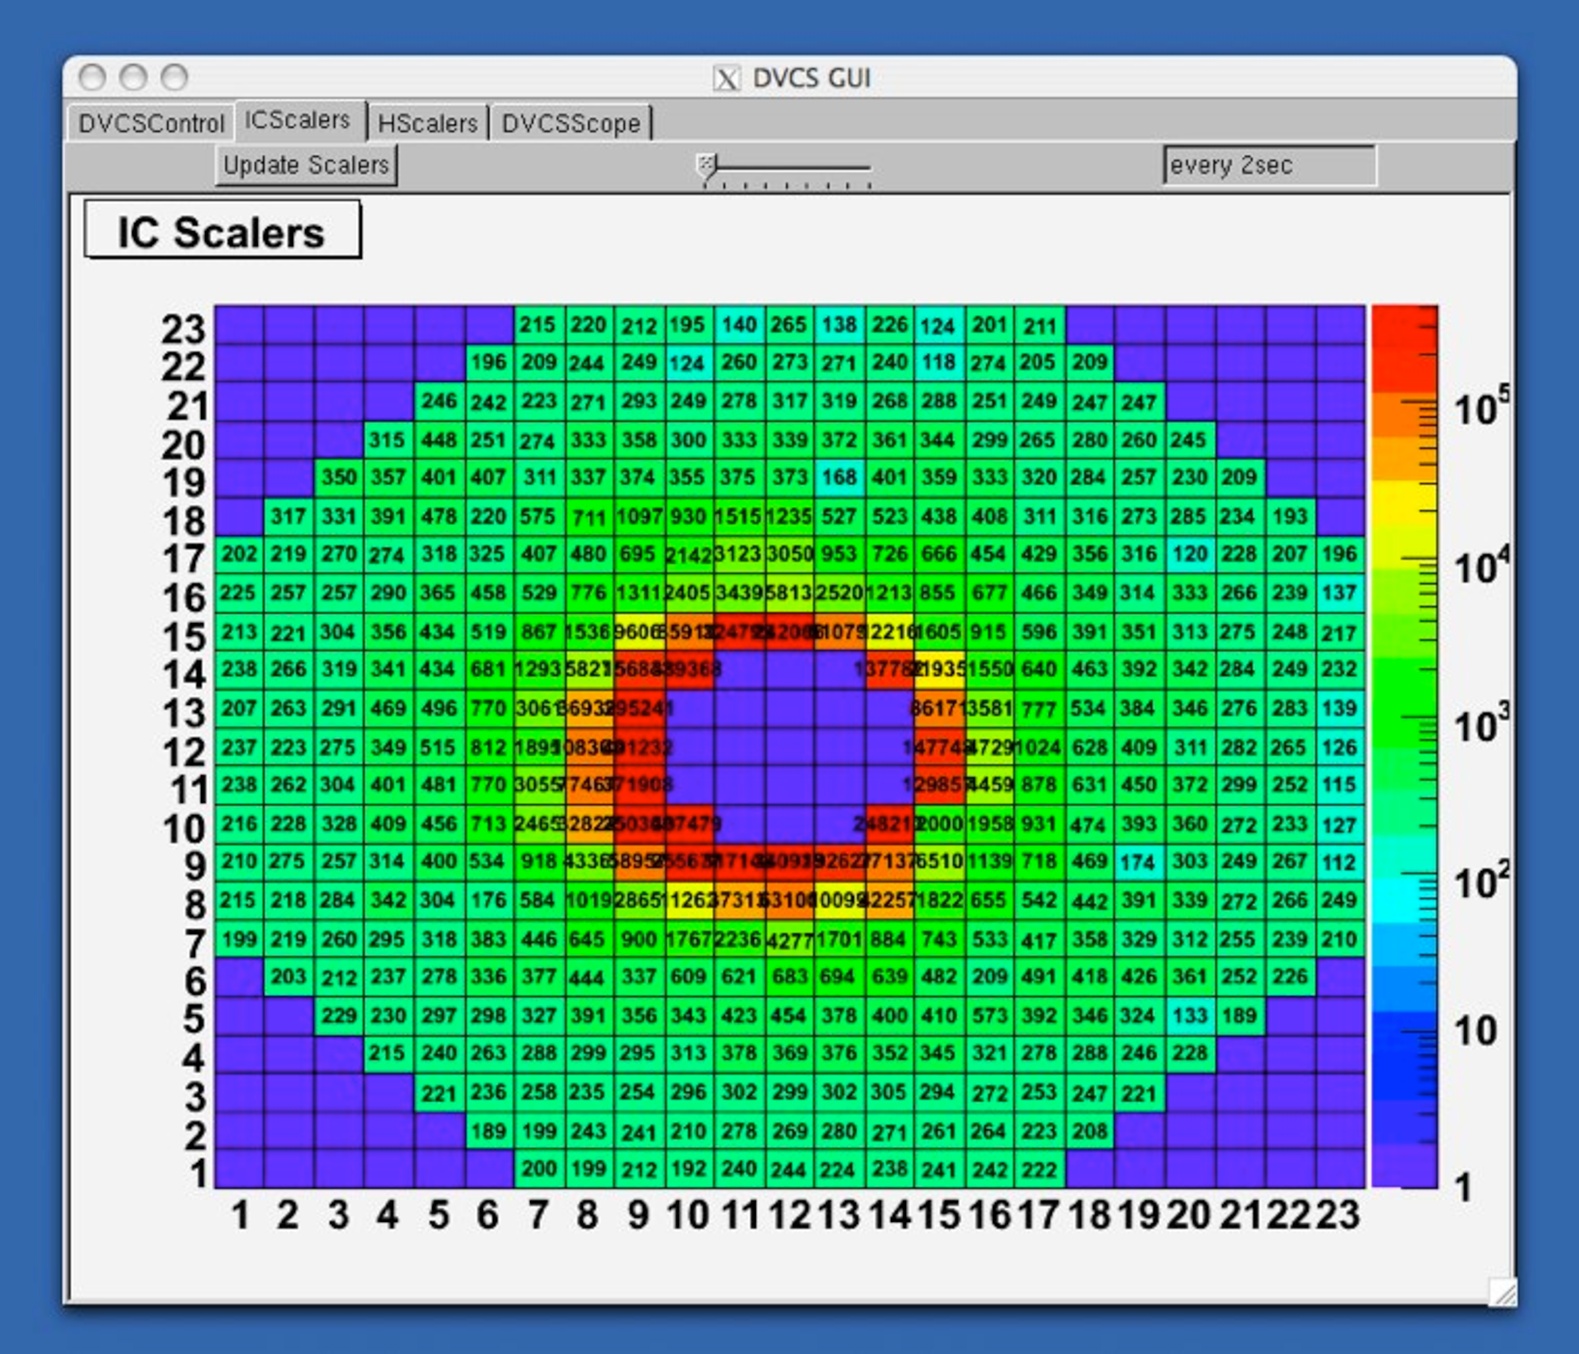
\includegraphics[scale=0.6]{daq_trigger/figures/dvcs_beam}
\caption{\small{Scalers (example from the previous version of the calorimeter).}}
\label{fig:dvcs_beam}
\end{figure}
Diagnostic scope permits to analyze on-line  the trigger logic. The goal to have  the Two-Dimensional Analyzer
 is to provide a remote debug interface to identify bad channels, verify cluster finding algorithms and check timing.
 The details of this analyzer are as following:
 
\begin{itemize}
\item Logic analyzer runs in parallel, non-intrusive, to the calorimeter trigger
\item Can setup trigger on any ECal pixel arrangement and/or cluster count
\item Can move forward/backward in time by ~250 ns to see timing details
\item Will be customize for HPS geometry and hardware
\end{itemize}

The example of the 2D analyzer is presented in Fig.~\ref{fig:dvcs_2_cluster}. Two clusters are displayed
in the picture. The red color displays the hits in the calorimeter and  the center of clusters is displayed in yellow.

In addition to the scalers, the distributions on individual ADC channel pulse energy will be provided.
The cluster hits positions and energy from SSP processor will be histogrammed as well. Two histograms (accepted and rejected) will be provided for each trigger cut used in the trigger logic.



\begin{figure}[t]
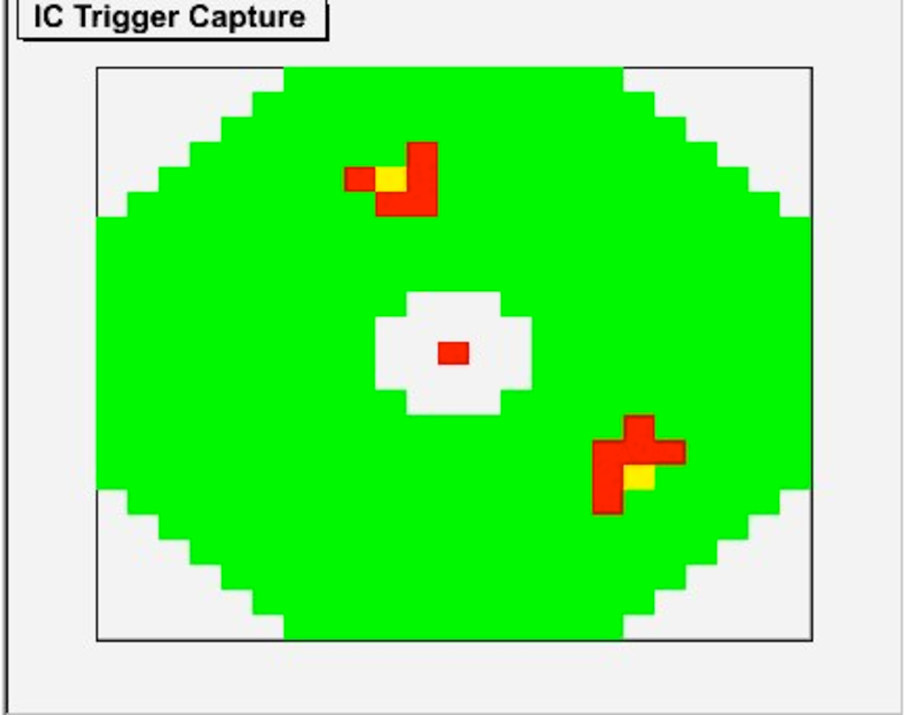
\includegraphics[scale=0.8]{daq_trigger/figures/dvcs_2_cluster}
\caption{\small{Diagnostic scope (example with two clusters found from the previous version of the calorimeter). Green - no hits, red - tower with hit, yellow - cluster found.}}
\label{fig:dvcs_2_cluster}
\end{figure}






%\subsubsection{Muon Trigger}
{\bf $\mu^+\mu^-$ Trigger} 

In similar manner, the muon trigger will look for MIP energy deposition in a single ECal channel and in the muon hodoscopes. CTPs in three VXS crates will collect MIP hits by using energy cuts on reported by FADCs hits, $E_{MIP}^{min}<E_{ECal\_channel}<E_{MIP}^{max}$ and $E_{MIP}<E_{\mu\_hodo}$. The CTP in the muon system VXS crate will use time information of reported MIP hits to select coincidences in two planes of each hodoscope layer according to the geometry of horizontal and vertical strips. After the MIP hits in ECal and in the muon system are selected, CTP sends the time and position information of each selected hit to SSP. The SSP first will look for time and position coincidence of MIP hits in ECal with at least two first layers of the muon system in each half of the detector separately (beam up and beam down), then for the $\mu^+\mu^-$ trigger it will select pairs of MIP hits in opposite sections of the detector (similar to the above described coplanarity requirements) that are within programable coincidence time window. 

